\section{Introduction}
  \label{sec:introduction}

High Performance Computing (HPC) systems have become critical infrastructures for science and industry. For example, domain experts use HPC systems to run large-scale physical simulations, big data analysis, multi-layer artificial neural networks, molecular dynamics experiments, and DNA sequencing.

As different HPC systems typically have customized software environments, HPC users must often configure and build their application for each specific machine, which is time consuming and can become a bottleneck to productivity. Moreover, in some cases, years- or even decades-old legacy applications still serve as key components in the process of scientific or industry research.  These legacy applications may have no active support and often require specific deprecated versions of libraries and/or hardware in order to make them run correctly. It may be hard to find or build library implementations that meet the requirement of legacy applications while remaining compatible with current HPC systems. These requirements impose great challenges for HPC users.  

%In a shared resource computing environment, users commonly implement checkpoint/restoration to stop and resume their computations across allocations, because of time or resource limitations. 



Due to availability of shared computing environment, users may need to frequently switch between computing systems. This can be among different HPC platforms or even cloud platforms. Differences in software environments may impede users when choosing a platform that has different software/hardware configurations. A consistent execution environment is also important for HPC application developers. Consistency between developing, testing, and production environments can greatly save developers' time on fixing compatibility issues, that can significantly accelerate the development process.



\begin{figure*}[h!]
%\vspace*{-1em}
    \centering
    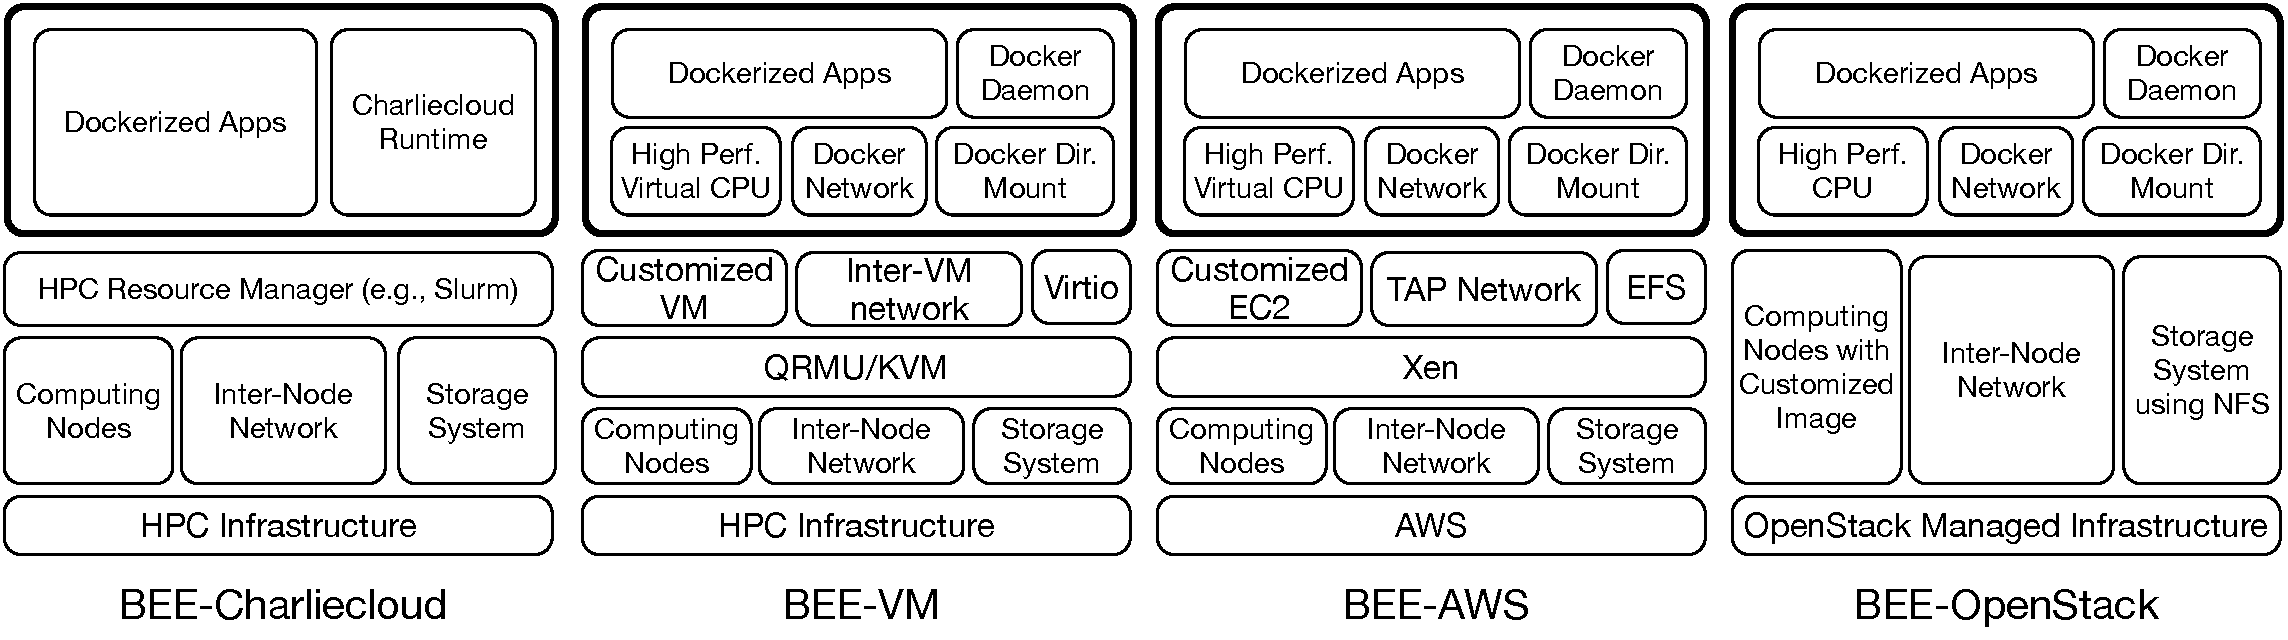
\includegraphics[width=0.8\textwidth]{figures/bee-framework-detail.pdf}
    \caption{BEE Backends}
    \label{bee-backend}
%\vspace*{-1em}
\end{figure*}


Virtualized environments, and particularly virtual machines (VMs), have been thoroughly investigated for HPC systems to provide more consistent, isolated, and secure environments \cite{vallee2008system, reuther2012hpc}. For example, Huang, et al. \cite{huang2006case} built a virtualized HPC environment using Xen-based VMs. By leveraging high performance I/O passthrough \cite{liu2006high}, VMs can achieve near-native performance when running HPC benchmarks. In \cite{zhang2016slurm}, Zhang, et al. illustrated that current resource managers in HPC systems cannot well supervise VMs and associated critical resources, so they proposed Slurm-V, that extends Slurm with virtualization-oriented capabilities. Huang, et al. and Tikotekar, et al. \cite{gugnani2016performance, tikotekar2008analysis} characterized the performance  of running multiple kinds of applications on virtualized HPC clusters. In \cite{huang2007virtual}, Huang, et al. proposed Inter-VM Communication (IVC), a VM-aware communication library to support efficient shared memory communication among computing processes on the same physical host and then they built an MPI library that was IVC enabled.

However, managing application specific VM images is not trivial, given that VM images need to contain files of the operating system, dependent libraries/packages, user applications, and input/output data, that may take several gigabytes of disk space. Migrating images between HPC systems or distributing images among compute nodes can consume a lot of time. On the other hand, Linux containers are more lightweight. Many implementations of Linux containers have been proposed e.g., Docker \cite{Docker}, Charliecloud \cite{priedhorsky2016charliecloud}, Shifter \cite{jacobsen2015contain}, and Singularity \cite{kurtzer_2016_60736}. They provide consistent execution environments for development, build, and deployment. By using Linux containers, developers only need to build their application once in the container on their local machine, and then the application can run on any supported machine. For doing that, one only needs to transfer the container image to the target execution machine. The container image usually only contains minimal operating system composition, application-dependent libraries/packages, and user applications, with much less space requirement than VM images \cite{boettiger2015introduction}. Also, since  Linux containers allow the guest application to share much of the host operating system including the Linux kernel, the performance penalty is small \cite{merkel2014docker, ruan2016performance}.



It can be of great benefit to bring the advantages of 
Linux containers, as realized in the cloud, to HPC users; however, HPC systems have support of Linux containers in a non-uniformed fashion. Some systems can natively support widely used Docker containers; Some systems run incompatible older Linux kernels that make them unable to support Linux containers \cite{harji2013our}. Some systems cannot support Docker containers but can support other Linux container implementations e.g., Charliecloud \cite{priedhorsky2016charliecloud}, Shifter \cite{jacobsen2015contain} and Singularity \cite{kurtzer_2016_60736}. This is challenging for HPC users who want to take the benefits of Linux containers and who already have their HPC applications running in Linux containers on one system and need to migrate to another one, since different Linux containers/runtimes are not mutually compatible with each other.  Even on an HPC/cloud system where a certain kind of Linux container is supported, running HPC applications still needs complicated configuration, since Linux containers, by their nature, are built for isolation, that is contrary to the sharing fashion adopted by HPC applications.


%Docker is not usually supported on current HPC systems. The main reason behind it is that Docker requires a privileged service and a Linux kernel version higher than 3.8, while Linux kernel versions on current HPC production systems are typically far behind this \cite{harji2013our}. 

%Especially for national security oriented research facilities, such as Los Alamos National Laboratory, it can take years of security and compatibility evaluation before their production HPC systems can upgrade Linux kernel. 

%Although HPC systems that run containers are being actively deployed using software such as Shifter \cite{jacobsen2015contain} and Singularity \cite{kurtzer_2016_60736}, BEE-VM's approach is complementary.  HPC systems that have been built and deployed with Shifter or Singularity can run containerized applications without a VM layer. However, containers must be built or adapted for Singularity and Shifter.  BEE-VM brings containerized applications to other HPC machines and, because it runs Docker natively, does not require a rebuild when moving applications across machines. 

In this work, we design a unified build and execution environment that overcomes the challenges when running containerized applications in HPC systems.  We call it Build and Execution Environment (\texttt{BEE}). 



\begin{enumerate}
\item \textbf{Docker image support:} Among all kinds of Linux container implementations, Docker is one of the most widely used implementations in the HPC community. With the support of Docker image, current HPC users can deploy their Dockerized application using \texttt{BEE} with no modification.
\item \textbf{Reproducibility:}
\texttt{BEE} aims to build up similar HPC-friendly execution environments across different platforms, allowing Dockerized applications to behave consistently. This is accomplished through a series of specially design modules -- \texttt{BEE backends}. Different \texttt{BEE backends} target different classes of platform, but they can build up execution environments with similar hardware configuration and software stack.
\item \textbf{Multiple platforms support:}
We design four \texttt{BEE backends} that support four different classes of systems. For HPC systems, instead of using Docker container runtime, we choose to use Charliecloud, a Linux container implementation with much less usage requirement than Docker and its runtime supports running Docker images. Charliecloud only needs execution systems to have Linux user namespace enabled, and it is usually enabled by default on many current and new HPC systems. Using Charliecloud, we build our first \texttt{BEE backend} for HPC systems -- \texttt{BEE-Charliecloud}. For older HPC systems that do not have Linux user namespace support, \texttt{BEE} provides another \texttt{BEE backend} -- \texttt{BEE-VM}. It can run Dockerized HPC applications through Docker runtime via a specialized VM. In addition to HPC systems, we also design two \texttt{BEE backends} to support running HPC applications on cloud systems. These allow users to run HPC applications when cloud platforms are preferable computing resources for users. Specifically, \texttt{BEE} provides \texttt{BEE-AWS} that allows Dockerized HPC applications to run on Amazon Web Services (AWS) platform and \texttt{BEE-OpenStack} for OpenStack-based HPC or cloud infrastructures. 
\item \textbf{End-to-end automation:}
\texttt{BEE} provides end-to-end automation that hides all launching details from users. Users only need to provide a \texttt{BEE} task description file (\texttt{beefile}), Docker images, and run scripts in order to launch a task on \texttt{BEE}. \texttt{BEE} will handle all the complications including: connecting to the remote platform, setting up suitable computing environment, configuring network and storage, and launching applications.
\item \textbf{Flexibility:}
\texttt{BEE} provides a unified user interface, so together with \texttt{BEE backends}, \texttt{BEE} users have the flexibility to switch between different platforms, as their needs require, with no modification to their applications and minimum modification to the task description file.
\end{enumerate}

\begin{figure*}[t]
%\vspace*{-1em}
    \centering
    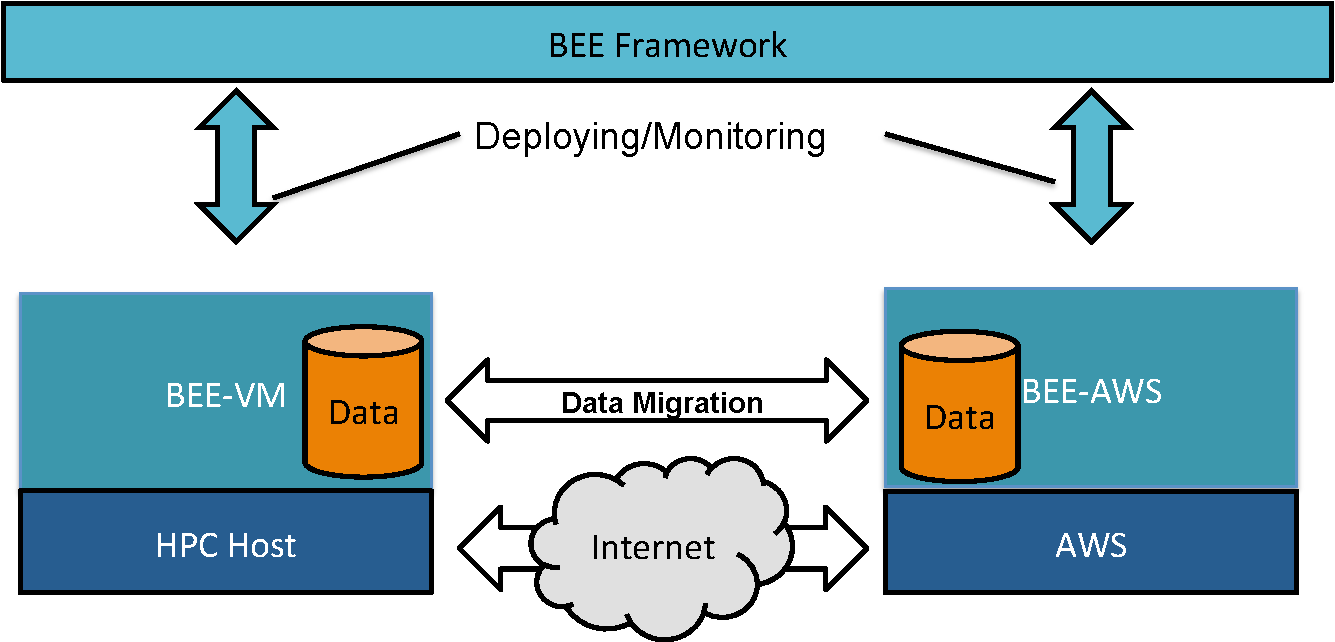
\includegraphics[width=0.8\textwidth]{figures/bee-framework.pdf}
    \caption{BEE Framework}
    \label{bee-framework}
%\vspace*{-1em}
\end{figure*} 


The rest of this paper is organized as follows:  
We discuss the BEE framework design in section \ref{bee-framework-section}. The designs of four \texttt{BEE backends} are discussed in section \ref{bee-charliecloud-section} - \ref{bee-openstack-section}. Performance is evaluated in section \ref{evaluation-section}. We showcase VPIC, a real HPC application running in \texttt{BEE} in section \ref{case-study-section}. In section \ref{related-work-section}, we discuss related works and how \texttt{BEE} is unique. Finally, we make our conclusion in section \ref{conclusions-section}.





